\chapter{Introduction}

\section{Motivation and Objectives}

A long term goal of artificial intelligence (AI) is the development of artificial general intelligence (AGI). 	A number of theoretical frameworks have been presented as formalizations of what it means to achieve AGI, notably by Hutter \cite{Hutter2005}.

Reinforcement learning is fundamental in Hutter's framework, and, as of March 2016, deep reinforcement learning (DRL) systems have mastered a wide range of tasks, including wide range of Atari 2600 games and Go \cite{Mnih2015, Silver2016}.

Though DRL systems have been remarkably successful, they still have a number of drawbacks \cite{Garnelo2016}:

\begin{enumerate}
\item \textbf{Slow to learn}. Deep neural networks require large data sets and are therefore
slow to learn.
\item \textbf{Fail to transfer past experience}. They often fail to perform well on tasks very
similar to those they have mastered.
\item \textbf{Inability to reason abstractly}. They fail to exploit statistical regularities in the
training data by using high-level processes like planning or causal reasoning.
\item \textbf{Hard to reason about}. It's often difficult to understand why the DRL
system chose the action it did.
\end{enumerate}

\begin{figure}[h!]
\centering
\begin{minipage}{.45\textwidth}
  \centering
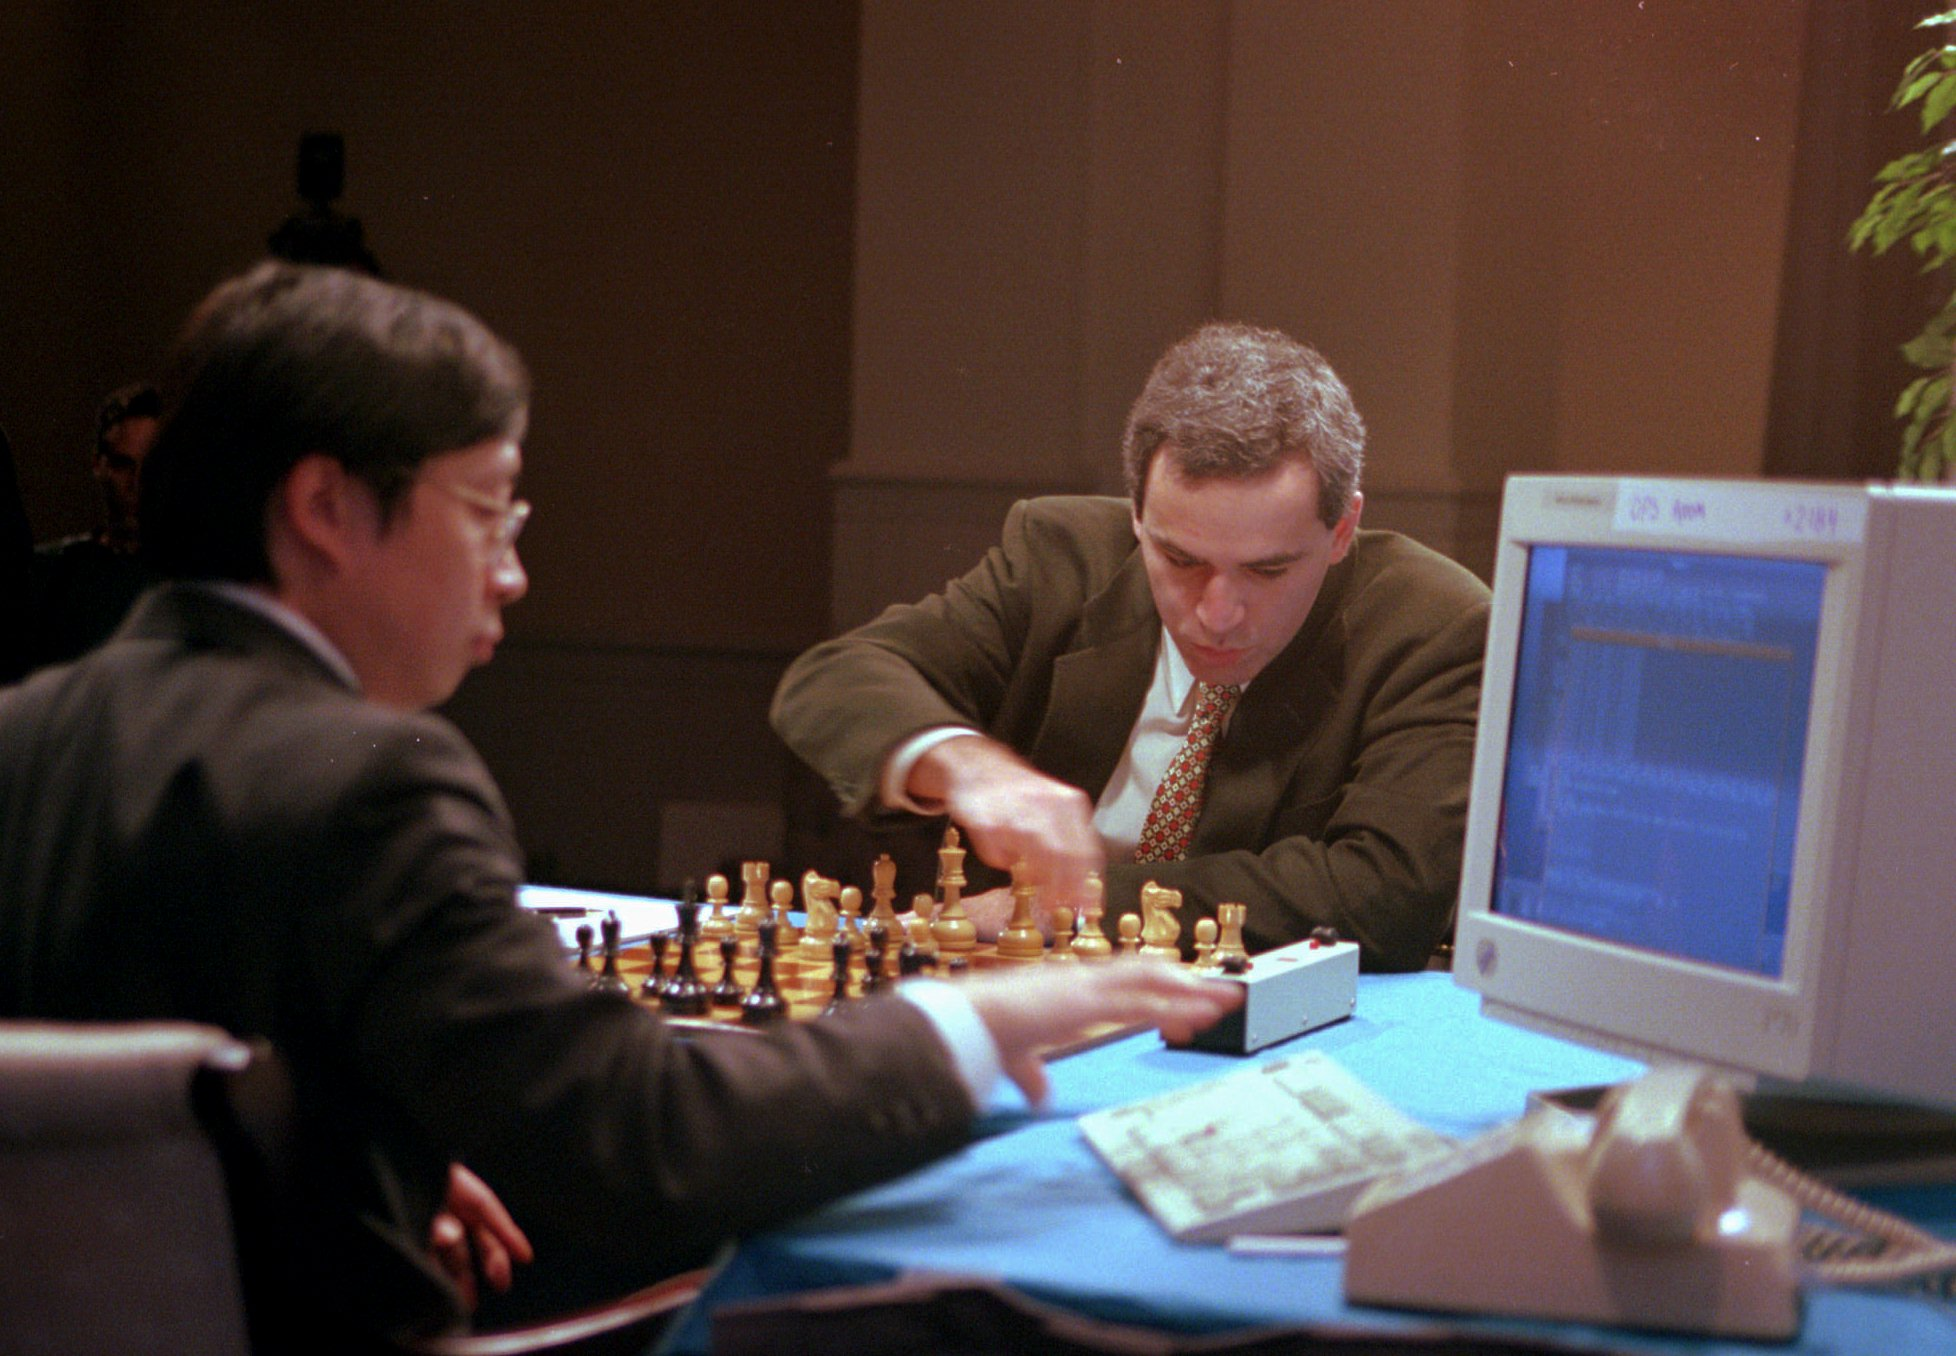
\includegraphics[width=\textwidth]{introduction/deep_blue_kasparov.jpg}
  \caption{May 1997: Gary Kasparov makes his first move against IBM's Deep Blue. Deep Blue would later emerge the victor in the best of six games; the first defeat of a reigning world chess champion by computer. \cite{Rosen2012}}
  \label{fig:deep_blue_kasparov}
\end{minipage}%
  \hfill
\begin{minipage}{.45\textwidth}
  \centering
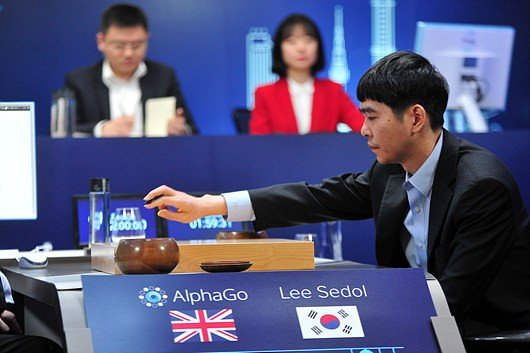
\includegraphics[width=\textwidth]{introduction/alpha_go_first_move_game_three.jpg}
  \caption{March 2016: Lee Sedol plays the first move of game three against AlphaGo. AlphaGo won four of five games. \cite{Ormerod2016}}
  \label{fig:alpha_go_first_move_game_three}
\end{minipage}
\end{figure}


Deep symbolic reinforcement learning (DSRL) is a recent advance which overcomes all of these drawbacks without the drawbacks from classical symbolic AI, namely the symbol grounding problem \cite{Garnelo2016}.

\begin{figure}[h!]
\centering
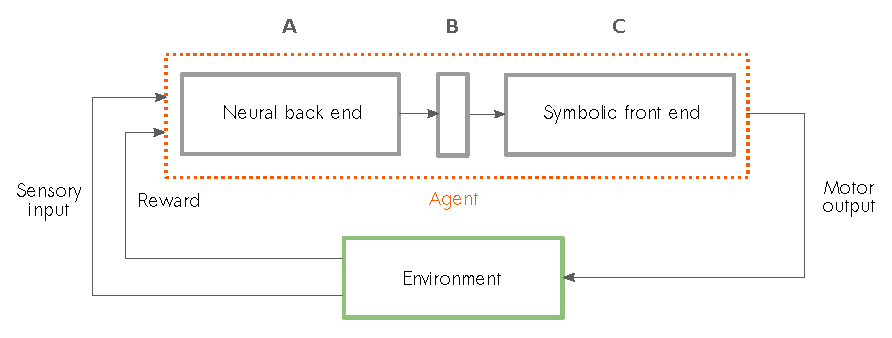
\includegraphics[width=\textwidth]{introduction/DSRL_architecture.eps}
\caption{Overview of deep symbolic reinforcement learning system architecture. \textbf{A}: The neural back end maps high-dimensional raw input data to a low-dimensional compositionally structured symbolic representation. \textbf{B}: The low-dimensional compositionally structured symbolic representation. \textbf{C}: Reinforcement learning of mapping from symbolic representation to action with maximum expected reward over time. \textit{Source: Garnelo et al.} \cite{Garnelo2016}.}
\label{fig:dsrl_archiecture}
\end{figure}

The architecture of the DSRL is shown in Figure \ref{fig:dsrl_archiecture}. The raw high-dimensional input, say an image, is mapped to a low-dimensional symbolic representation. This is done by passing the high-dimensional input through a series of convolutional layers and extracting the activation spectra in the latent space. These spectra are then used to classify the  

 relies on the unsupervised extraction of disentangled features, allowing for transfer learning and high-level cognitive processes. However, the unsupervised extraction of features from a wide range of scenes is still a challenge in AI research [? ]. Fortunately methods are getting better, and the first unsupervised scalable model $\beta$-VAE was developed recently.

\section{Contributions}

Contributions here.